\documentclass[pdftex,12pt,a4paper]{article}

\usepackage{float}
\usepackage{graphicx}  
\usepackage[margin=2.5cm]{geometry}
\usepackage{breakcites}
\usepackage{indentfirst}
\usepackage{pgfgantt}
\usepackage{pdflscape}
\usepackage{float}
\usepackage{epsfig}
\usepackage{epstopdf}
\usepackage[cmex10]{amsmath}
\usepackage{stfloats}
\usepackage{multirow}
\setcounter{section}{-1}
\usepackage[export]{adjustbox}% http://ctan.org/pkg/adjustbox
\usepackage[%
    pdfborder={0 0 0}
]{hyperref}
\usepackage{listings}
\lstset{frame=tb,
  language=Java,
  aboveskip=3mm,
  belowskip=3mm,
  showstringspaces=false,
  columns=flexible,
  basicstyle={\small\ttfamily},
  numbers=none,
  breaklines=true,
  breakatwhitespace=true,
  tabsize=3
}


\renewcommand{\refname}{REFERENCES}
\linespread{1.3}

\usepackage{mathtools}
%\newcommand{\HRule}{\rule{\linewidth}{0.5mm}}
\thispagestyle{empty}
\begin{document}
\begin{titlepage}
\begin{center}
\textbf{}\\
\textbf{\Large{ISTANBUL TECHNICAL UNIVERSITY}}\\
\vspace{0.5cm}
\textbf{\Large{COMPUTER ENGINEERING DEPARTMENT}}\\
\vspace{2cm}
\textbf{\Large{BLG 222E\\ COMPUTER ORGANIZATION\\ PROJECT REPORT}}\\
\vspace{2.8cm}
\begin{table}[ht]
\centering
\Large{
\begin{tabular}{lcl}
\textbf{PROJECT NO}  & : & 1 \\
\textbf{GROUP NO}  & : & G71 \\
\end{tabular}}
\end{table}
\vspace{1cm}
\textbf{\Large{GROUP MEMBERS:}}\\
\begin{table}[ht]
\centering
\Large{
\begin{tabular}{rcl}
150220901  & : & MOHAMAD CHAHADEH \\
150190068  & : & ÖZGÜR SEFEROĞLU \\
150200913  & : & FITNETE GUNI
\end{tabular}}
\end{table}
\vspace{2.8cm}
\textbf{\Large{SPRING 2023}}

\end{center}

\end{titlepage}

\thispagestyle{empty}
\setcounter{tocdepth}{4}
\tableofcontents
\clearpage

\section{Introduction}

\subsection{Project Parts}
\begin{itemize}
\item Part 1: n-bit register
\item Part 2: Register Files \begin{itemize}
\item Part 2a: 16-bit IR Register
\item Part 2b: Register File (RF)
\item Part 2c: Address Register File (ARF)
\end{itemize}
\item Part 3: 8-bit ALU
\item Part 4: Whole System Integration
\end{itemize}

\subsection{Task Distribution}
\begin{enumerate}
\item ÖZGÜR SEFEROĞLU:  Part 3, Part 4
\item MOHAMAD CHAHADEH:  Part 1, Part 2a, Part 2b, Part 4
\item FITNETE GUNI: Part 2c
\end{enumerate}

\pagebreak

\section{Part 1}
Implementing an n-bit Register, controlled using a 2-bit FunSel signal and an Enable signal. \hyperref[fig:part1_char]{Figure \ref{fig:part1_char}} Shows the diagram and characteristic equation of Part 1.

\begin{figure}[H]
\centering
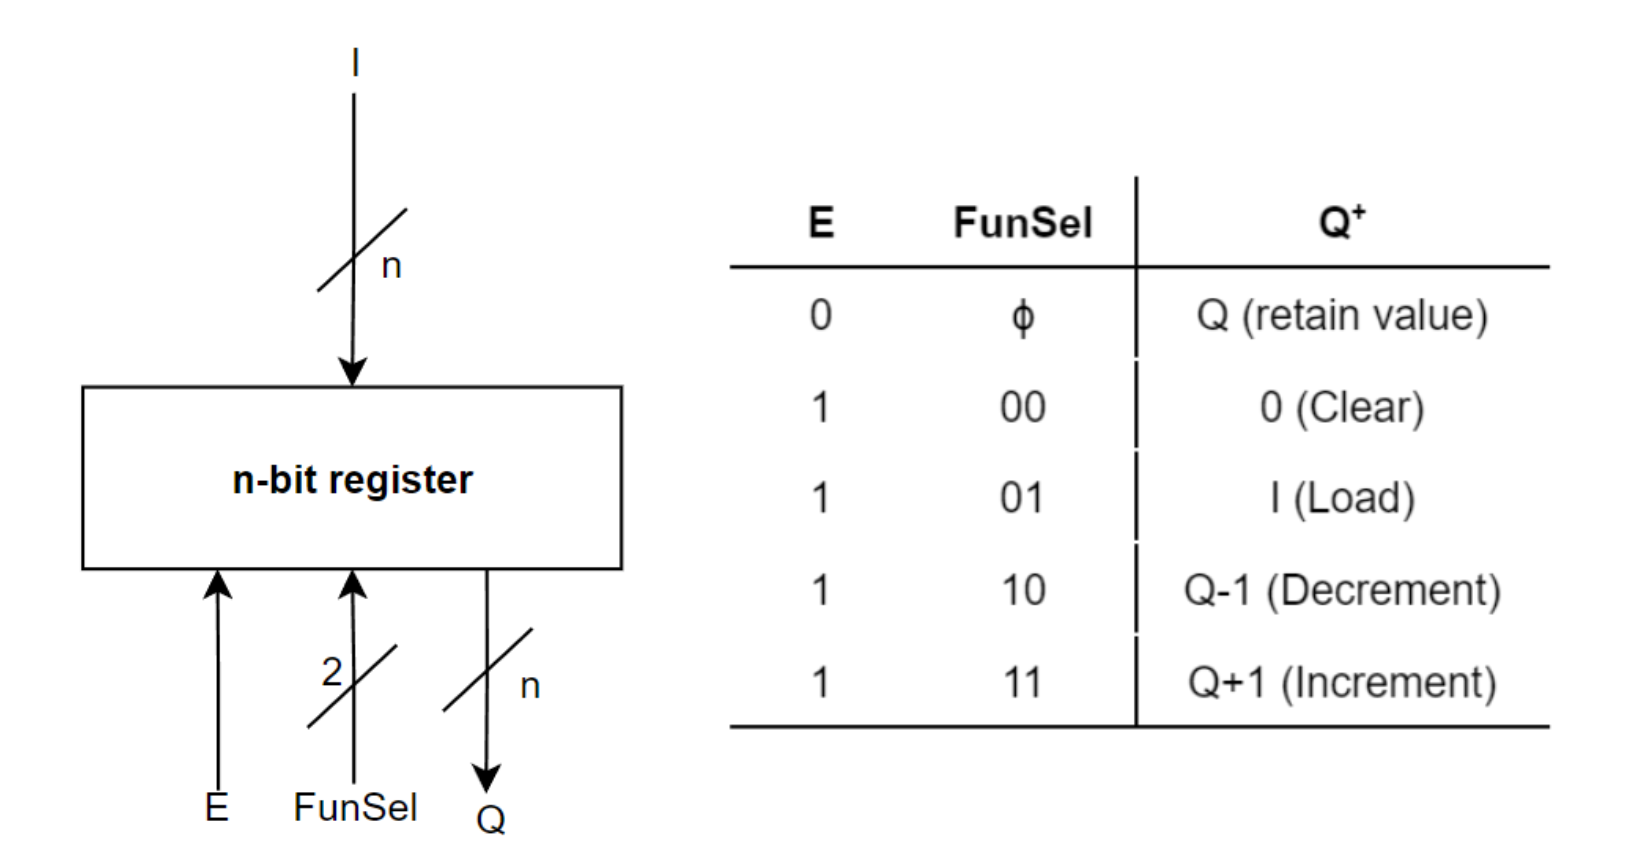
\includegraphics[width=0.7\textwidth]{part1_diagram.png}
\caption{Diagram and characteristic equation of Part 1}
\label{fig:part1_char}
\end{figure}

\subsection{Implementation}
the module implemented takes one parameter n, which is the number of bits of the register, a clock signal, two control inputs being FunSel and Enable, and one output of n-bits. the module is implemented by use the always block which executes on every positive edge of the clock, an if statement to check the enable signal, and a case block for the various inputs of FunSel. the following is the code for implementing the module.
\vspace{0.7cm}

\begin{lstlisting}
module part1 #(parameter n = 4) 
(input clk,
 input [1:0] FunSel,
 input [n-1:0] data_in, 
 input enable, 
 output reg [n-1:0] data_out);

    wire [n-1:0] zero = 0;
    always @(posedge clk)
    begin
        if (enable == 0)
            data_out <= data_out;
        else
            case (FunSel)
                2'b00: data_out <= zero;
                2'b01: data_out <= data_in;
                2'b10: data_out <= data_out - 1;
                2'b11: data_out <= data_out + 1;
            endcase
    end
endmodule
\end{lstlisting}

\subsection{Simulation}
\hyperref[fig:part1_sim]{Figure \ref{fig:part1_sim}} Shows a simulation of the module implemented earlier of n = 4.
\begin{figure}[H]
\centering
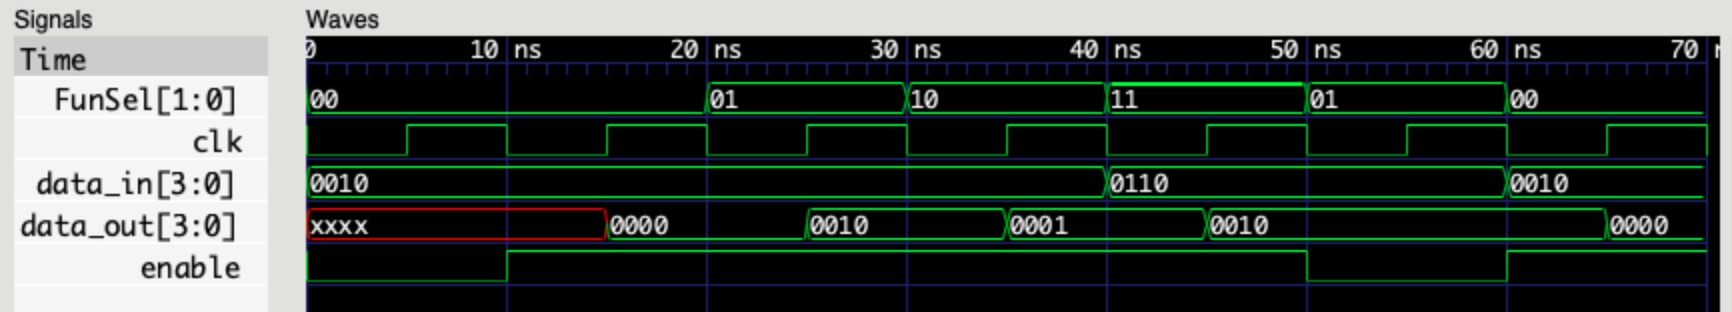
\includegraphics[width=1\textwidth]{part1_sim.png}
\caption{Simulation of Part 1, n-bit Register.}
\label{fig:part1_sim}
\end{figure}

\section{Part 2}

\subsection{Part 2a}
Designing a 16-bit IR Register whose Diagram and Characteristic table is shown in \hyperref[fig:part2a_diagram]{Figure \ref{fig:part2a_diagram}}.

\begin{figure}[H]
\centering
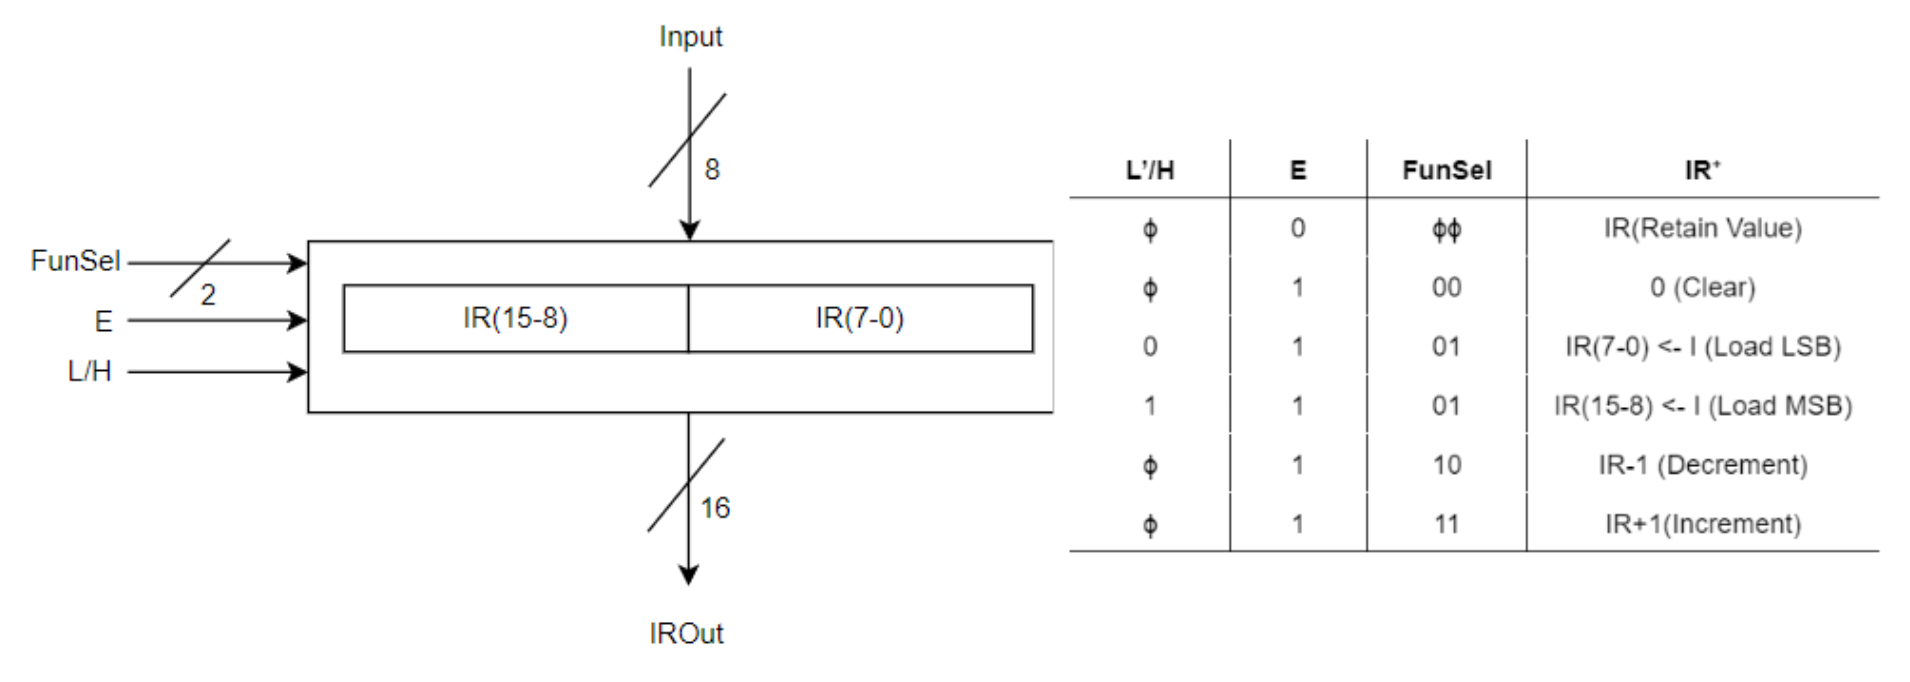
\includegraphics[width=0.7\textwidth]{part2a_diagram.png}
\caption{Diagram and Characteristics of Part 2a}
\label{fig:part2a_diagram}
\end{figure}

\subsubsection{Implementation}
To implement the IR register in Verilog, we need 1 data input and 3 control signals, it can be implemented as follows:

\begin{lstlisting}
module part2a_IRreg(input clk, input[7:0] I, input [1:0] FunSel, input LH, input enable, output reg [15:0] data_out);

    always @(posedge clk)
    begin
        if (enable == 0)
            data_out = data_out;
        else
            if(FunSel == 2'b00) data_out = 16'b000000000000000;
            else if(FunSel == 2'b01) begin
                if(LH == 0) data_out[7:0] = I;
                else if(LH == 1) data_out[15:8] = I;
            end
            else if(FunSel == 2'b10) data_out = data_out - 1;
            else if(FunSel == 2'b11) data_out = data_out + 1;
    end

endmodule
\end{lstlisting}

\subsubsection{Simulation}
\hyperref[fig:part2a_sim]{Figure \ref{fig:part2a_sim}} Shows the simulation for the IR register implemented in this part.

\begin{figure}[H]
\centering
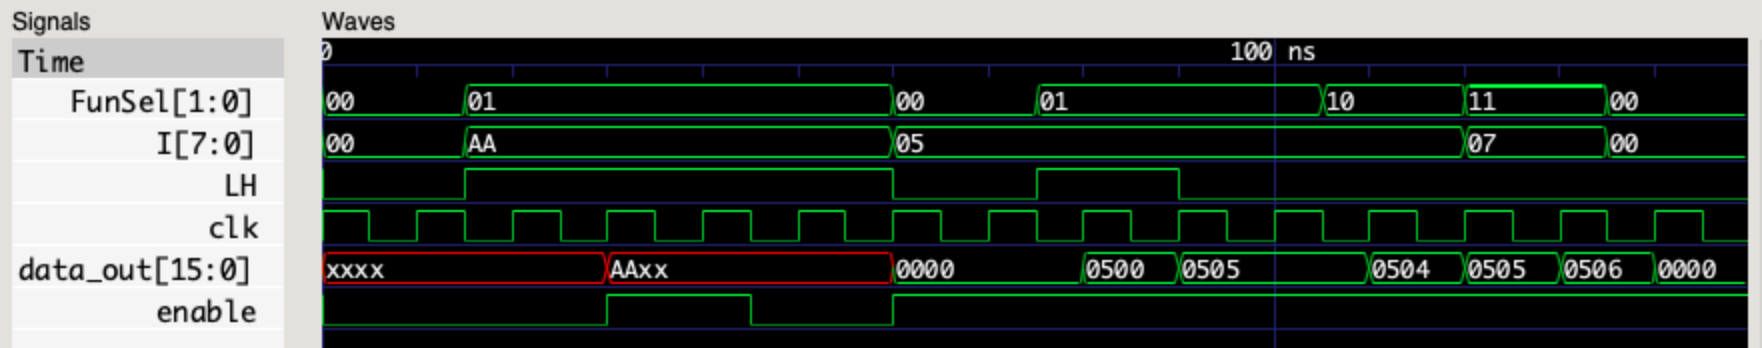
\includegraphics[width=1\textwidth]{part2a_sim.png}
\caption{Simulation of part2a}
\label{fig:part2a_sim}
\end{figure}

\subsection{Part 2b}
Implementing a Register file with 4 General Registers and 4 Temporary Register with the following diagram and characteristics:
\begin{figure}[H]
\centering
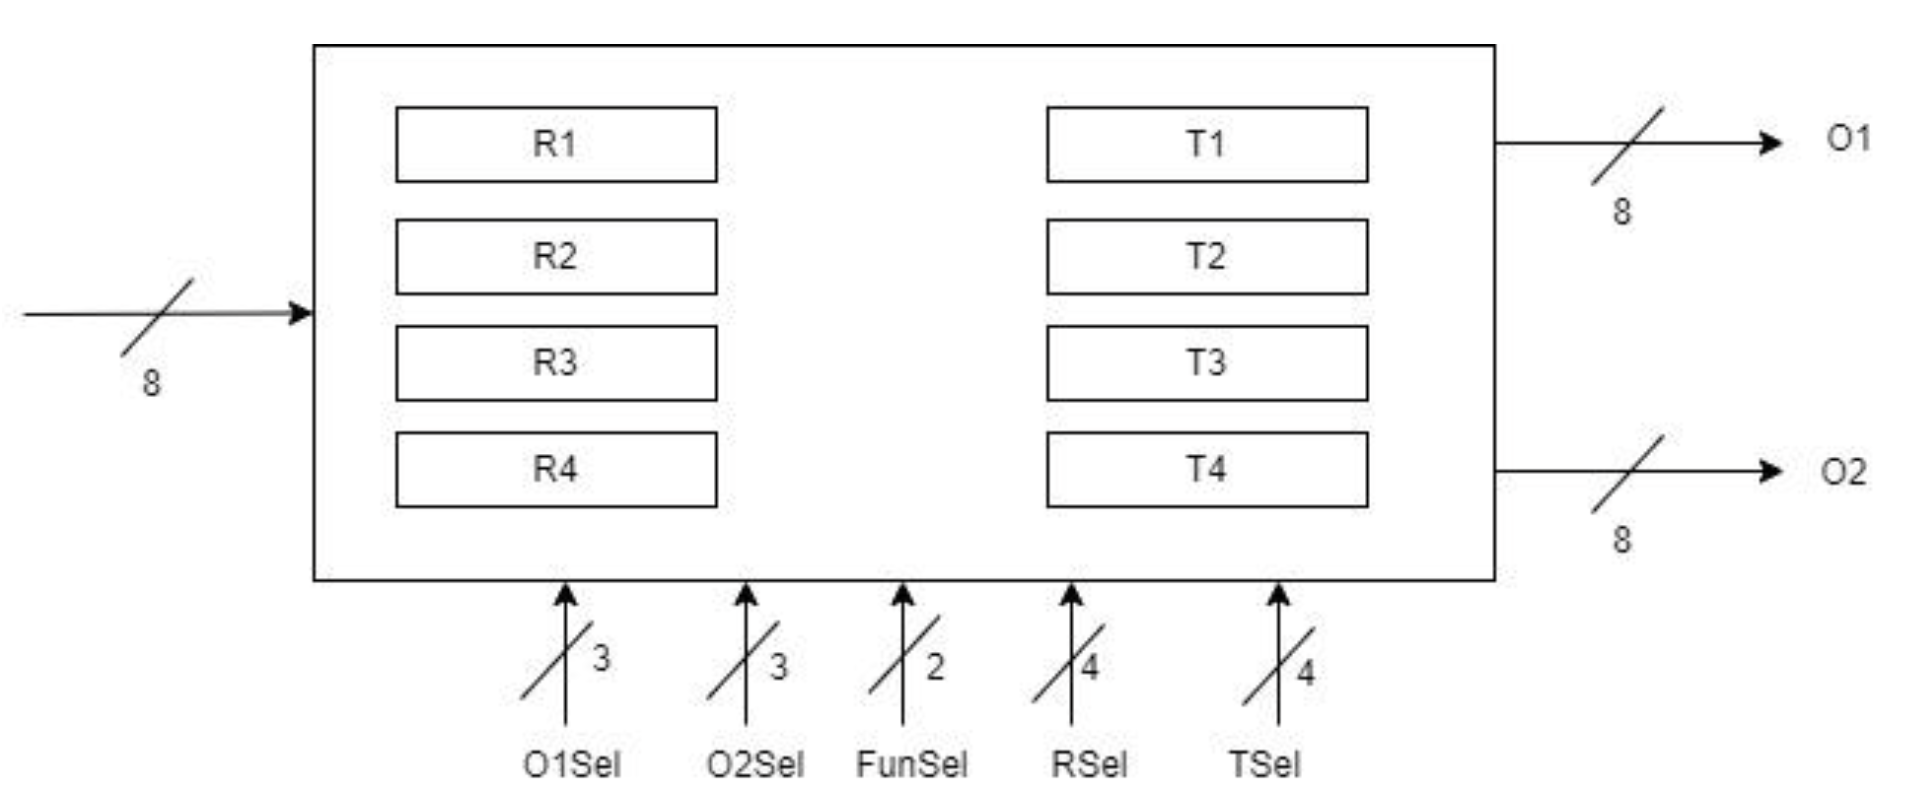
\includegraphics[width=0.5\textwidth, valign=c]{part2b_diagram_2.png}
\hspace{1cm}
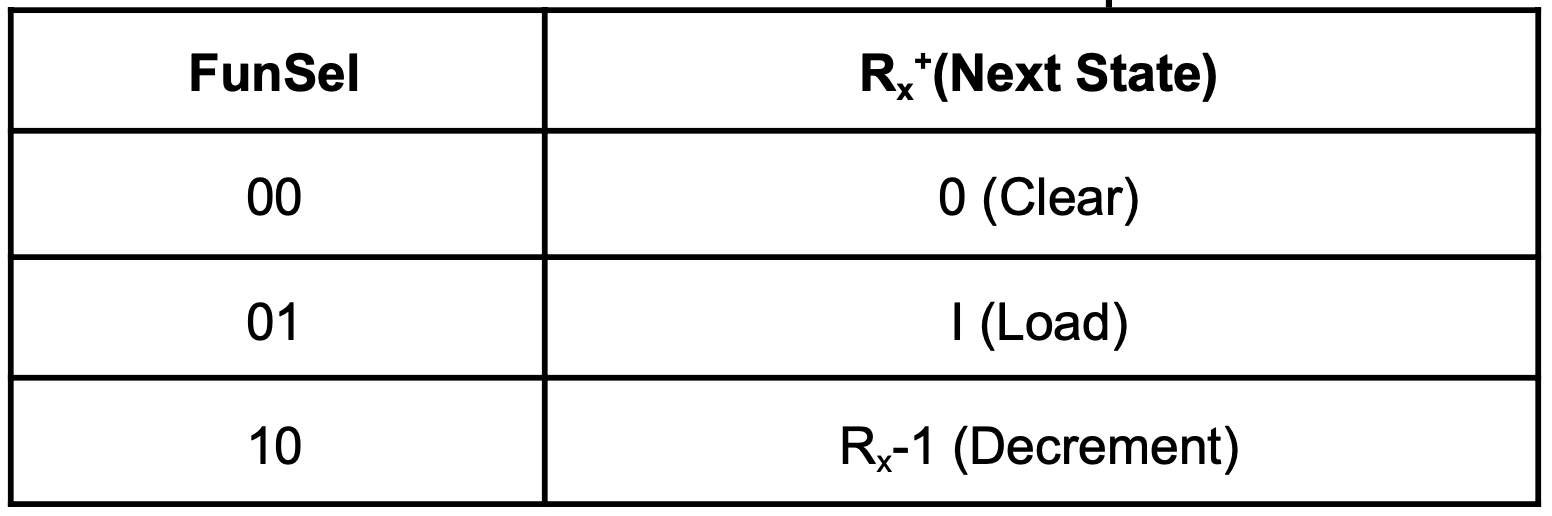
\includegraphics[width=0.3\textwidth, valign=c]{part2b_diagram_1.png}
\caption{Diagram of Part 2b}
\label{fig:part2b_diagram}
\end{figure}

\subsubsection{Implementation}
The Register File implemented Takes in 6 inputs:
\begin{itemize}
\item A single 8-bit data input.
\item O1Sel and O2Sel Output Control signals.
\item FunSel Function control signal.
\item RSel Register activation signal.
\item TSel Temporary Register activation signal.
\end{itemize}
And it is implemented as follows:

\begin{lstlisting}
module part2b ( input clk, input [7:0] I, input [2:0] O1Sel, input [2:0] O2Sel, input [1:0] FunSel, input [3:0] RSel, input [3:0] TSel, output reg [7:0] O1, O2 );

    reg [7:0] R1;
    reg [7:0] R2;
    reg [7:0] R3;
    reg [7:0] R4;
    
    reg [7:0] T1;
    reg [7:0] T2;
    reg [7:0] T3;
    reg [7:0] T4;
 
    always @ (posedge clk) begin

        if(FunSel == 2'b00) begin
            if(RSel[0] == 1) 
                 R4 = 8'b00000000;
            if(RSel[1] == 1) 
                 R3 = 8'b00000000;
            if(RSel[2] == 1) 
                 R2 = 8'b00000000;
            if(RSel[3] == 1) 
                 R1 = 8'b00000000;
            if(TSel[0] == 1) 
                 T4 = 8'b00000000;
            if(TSel[1] == 1) 
                 T3 = 8'b00000000;
            if(TSel[2] == 1) 
                 T2 = 8'b00000000;
            if(TSel[3] == 1) 
                 T1 = 8'b00000000;
        end
        else if(FunSel == 2'b01) begin
            if(RSel[0])  R4 = I;
            if(RSel[1])  R3 = I;
            if(RSel[2])  R2 = I;
            if(RSel[3])  R1 = I;
            if(TSel[0])  T4 = I;
            if(TSel[1])  T3 = I;
            if(TSel[2])  T2 = I;
            if(TSel[3])  T1 = I;
        end
        else if(FunSel == 2'b10) begin
            if(RSel[0])  R4 = R4 - 1;
            if(RSel[1])  R3 = R3 - 1;
            if(RSel[2])  R2 = R2 - 1;
            if(RSel[3])  R1 = R1 - 1;
            if(TSel[0])  T4 = T4 - 1;
            if(TSel[1])  T3 = T3 - 1;
            if(TSel[2])  T2 = T2 - 1;
            if(TSel[3])  T1 = T1 - 1;
        end
        else if(FunSel == 2'b11) begin
            if(RSel[0])  R4 = R4 + 1;
            if(RSel[1])  R3 = R3 + 1;
            if(RSel[2])  R2 = R2 + 1;
            if(RSel[3])  R1 = R1 + 1;
            if(TSel[0])  T4 = T4 + 1;
            if(TSel[1])  T3 = T3 + 1;
            if(TSel[2])  T2 = T2 + 1;
            if(TSel[3])  T1 = T1 + 1;
        end
                
        if( O1Sel == 3'b000)  O1 = T1;
        else if( O1Sel == 3'b001)  O1 = T2;
        else if( O1Sel == 3'b010)  O1 = T3;
        else if( O1Sel == 3'b011)  O1 = T4;
        else if( O1Sel == 3'b100)  O1 = R1;
        else if( O1Sel == 3'b101)  O1 = R2;
        else if( O1Sel == 3'b110)  O1 = R3;
        else if( O1Sel == 3'b111)  O1 = R4;


        if( O2Sel == 3'b000)  O2 = T1;
        else if( O2Sel == 3'b001)  O2 = T2;
        else if( O2Sel == 3'b010)  O2 = T3;
        else if( O2Sel == 3'b011)  O2 = T4;
        else if( O2Sel == 3'b100)  O2 = R1;
        else if( O2Sel == 3'b101)  O2 = R2;
        else if( O2Sel == 3'b110)  O2 = R3;
        else if( O2Sel == 3'b111)  O2 = R4;

    end 
endmodule
\end{lstlisting}

\subsubsection{Simulation}
\begin{figure}[H]
\centering
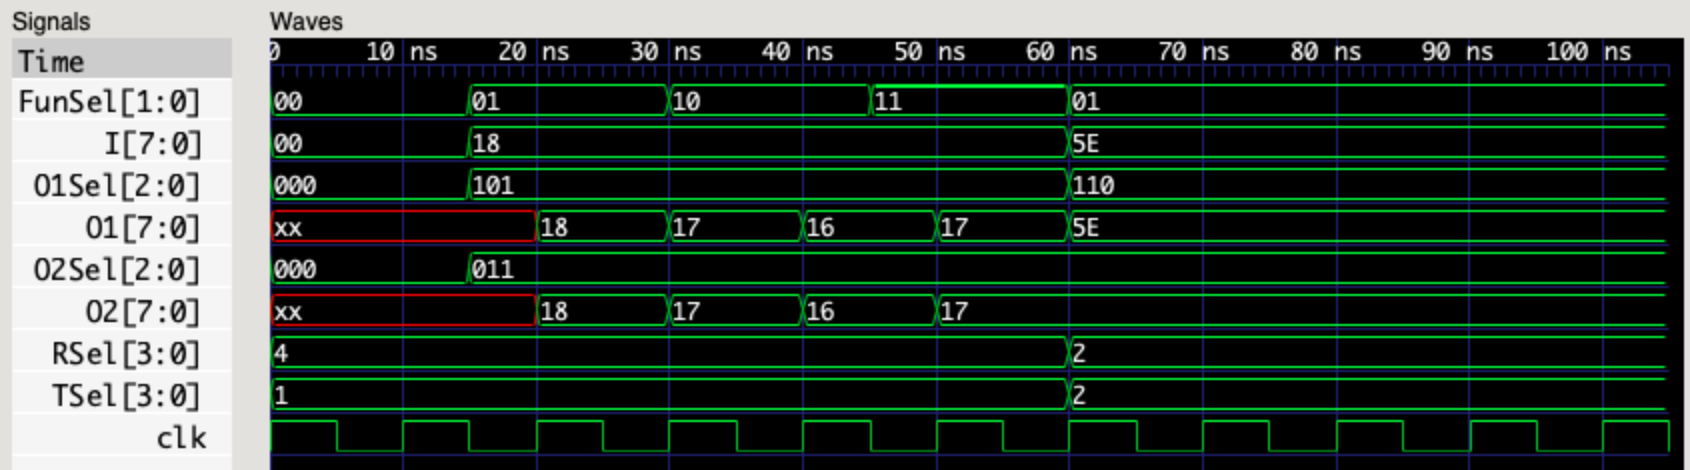
\includegraphics[width=1\textwidth]{part2b_sim.png}
\caption{Simulation of Part2b, Register File}
\label{fig:part2b_sim}
\end{figure}

\subsection{Part 2c}
an Address Register File which consists of four 8-bit address registers as shown in \hyperref[fig:part2c_diagram]{Figure \ref{fig:part2c_diagram}}.
\begin{figure}[H]
\centering
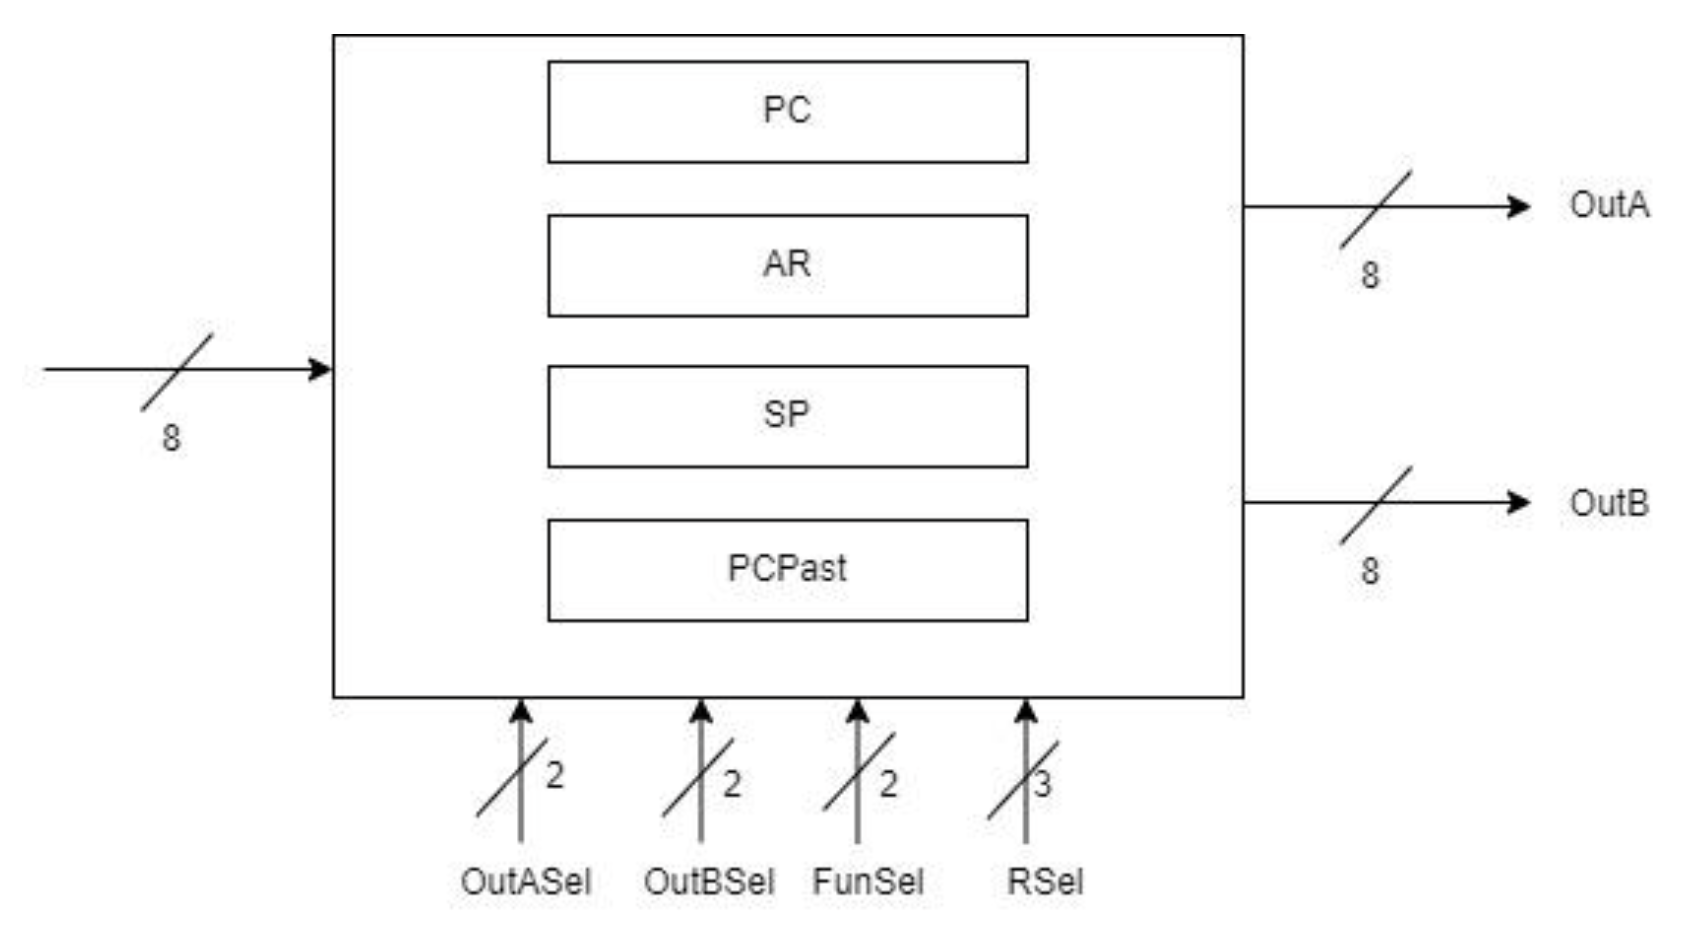
\includegraphics[width=0.7\textwidth]{part2c_diagram.png}
\caption{Diagram of Part 2c, Address Register File}
\label{fig:part2c_diagram}
\end{figure}
This Register will use the same Characteristic function as the previous part.

\subsubsection{Implementation}
The Address Register File implemented Takes in 6 inputs:
\begin{itemize}
\item A single 8-bit data input.
\item OutASel and OutBSel Output Control signals.
\item FunSel Function control signal.
\item RSel Register activation signal.
\end{itemize}
it is implemented in verilog as such:

\begin{lstlisting}
module part2c_ARF( input clk, input [7:0] I, input [1:0] OutASel, input [1:0] OutBSel, input [1:0] FunSel, input [3:0] RSel, output reg [7:0] OutA, output reg [7:0] OutB);

reg [7:0] PC;
reg [7:0] AR;
reg [7:0] SP;
reg [7:0] PCPast;


always @ (posedge clk) begin

    if(FunSel == 2'b00)
    begin
        if(RSel[3] == 1) 
            PC = 8'b00000000;
        if(RSel[2] == 1) 
            AR = 8'b00000000;
        if(RSel[1] == 1) 
            SP = 8'b00000000;
        if(RSel[0] == 1) 
            PCPast = 8'b00000000;
    end
    else if(FunSel == 2'b01)
    begin
        if(RSel[3] == 1) 
            PC = I;
        if(RSel[2] == 1) 
            AR = I;
        if(RSel[1] == 1) 
            SP = I;
        if(RSel[0] == 1)
            PCPast = I;
    end
    else if(FunSel == 2'b10)
    begin
        if(RSel[3] == 1) 
            PC = PC + 1;
        if(RSel[2] == 1) 
            AR = AR + 1;
        if(RSel[1] == 1) 
            SP = SP + 1;
        if(RSel[0] == 1)
            PCPast = PCPast + 1;
    end
    else if(FunSel == 2'b11)
    begin
        if(RSel[3] == 1) 
            PC = PC - 1;
        if(RSel[2] == 1) 
            AR = AR - 1;
        if(RSel[1] == 1) 
            SP = SP - 1;
        if(RSel[0] == 1)
            PCPast = PCPast - 1;
    end


    if(OutASel == 2'b00) OutA = AR;
    else if(OutASel == 2'b01) OutA = SP;
    else if(OutASel == 2'b10) OutA = PCPast;
    else if(OutASel == 2'b11) OutA = PC;

    if(OutBSel == 2'b00) OutB = AR;
    else if(OutBSel == 2'b01) OutB = SP;
    else if(OutBSel == 2'b10) OutB = PCPast;
    else if(OutBSel == 2'b11) OutB = PC;

end

endmodule
\end{lstlisting}

\subsubsection{Simulation}
\begin{figure}[H]
\centering
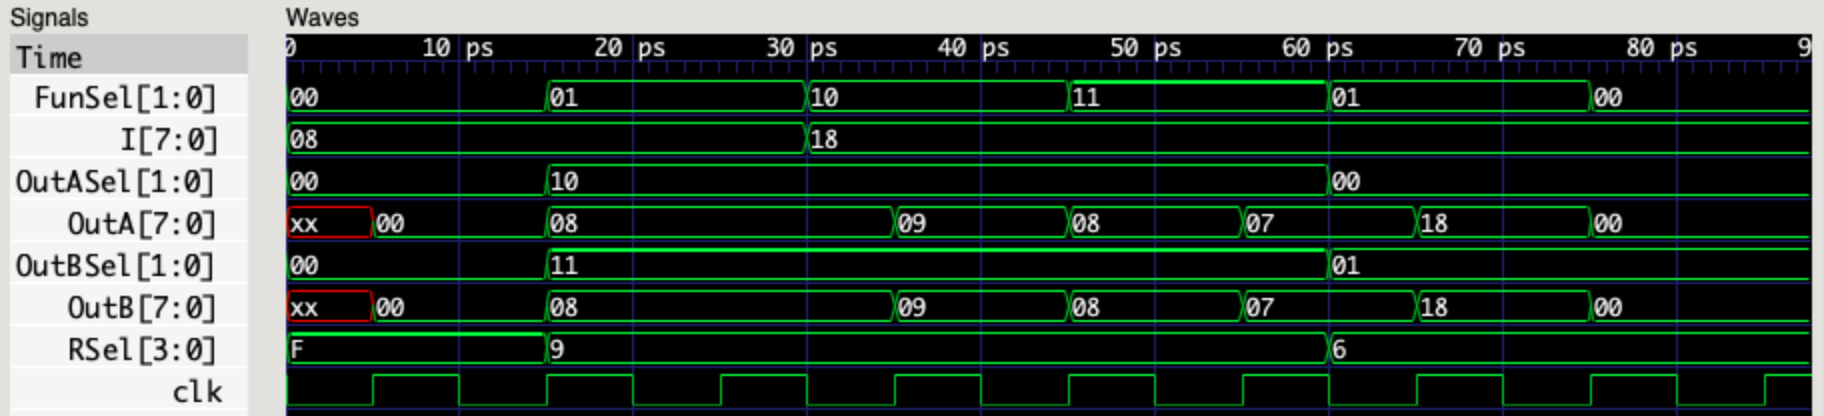
\includegraphics[width=1\textwidth]{part2c_sim.png}
\caption{Simulation of Part 2c, address Register File}
\label{fig:part2c_sim}
\end{figure}
\pagebreak


\section{Part 3}
Implementing an 8-bit ALU Module that does the following:
\begin{figure}[H]
\centering
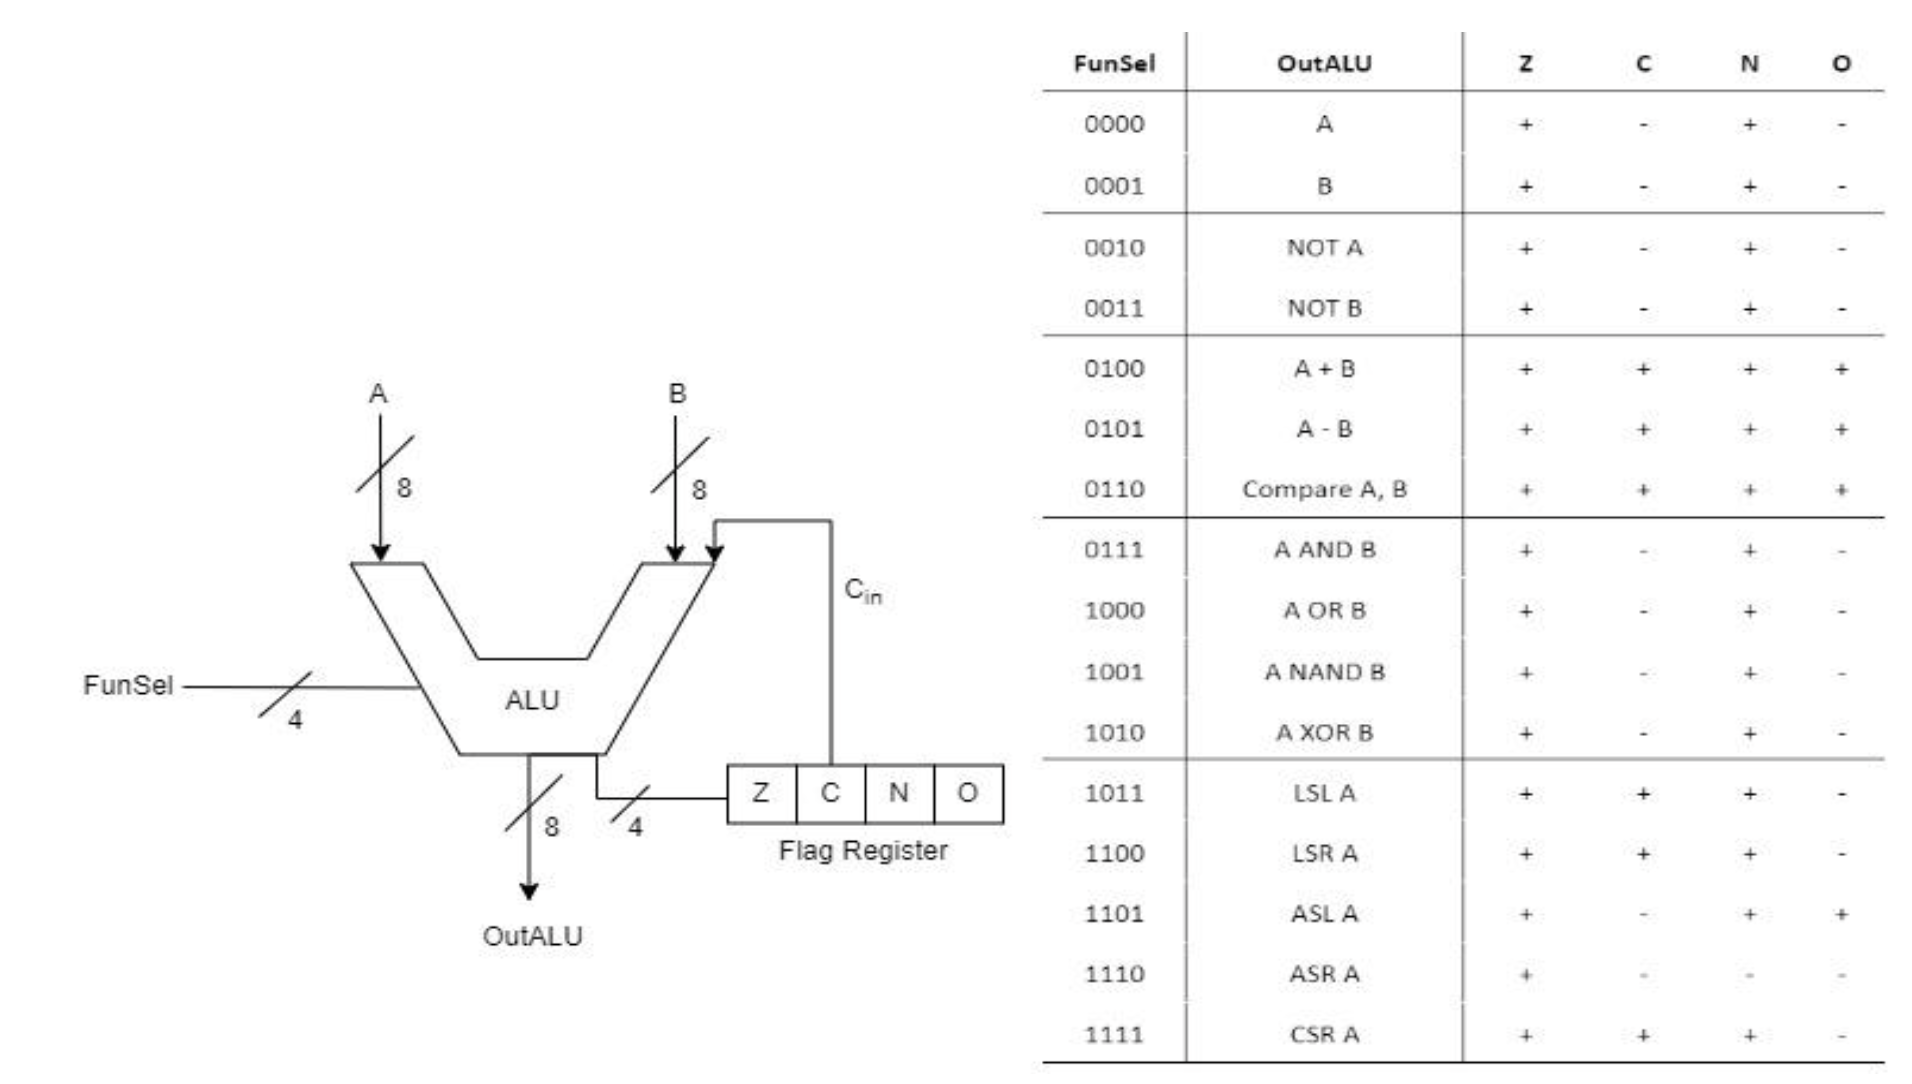
\includegraphics[width=1\textwidth]{part3_diagram.png}
\caption{Diagram of ALU module and its characteristics}
\label{fig:part3_diagram}
\end{figure}

\subsection{Implementation}
\begin{lstlisting}
module part3_ALU (input clk, input [7:0] A, input [7:0] B, input [3:0] FunSel, output reg [7:0] OutALU, output reg [3:0] Flags);

    reg [7:0] B_neg;
    reg cout;

    always @(posedge clk) begin
        B_neg = (~B) + 8'b00000001; // 2's complement of B
        cout = Flags[2];

        if(FunSel == 4'b0000)
            OutALU = A;
        else if(FunSel == 4'b0001)
            OutALU = B;
        else if(FunSel == 4'b0010)
            OutALU = ~A;
        else if(FunSel == 4'b0011)
            OutALU = ~B;
        else if(FunSel == 4'b0100) begin // A+B
            {cout, OutALU} = {1'b0, A} + {1'b0, B};
            if(cout == 1) Flags[0] = 1;
            else Flags[0] = 0;
        end
        else if(FunSel == 4'b0101)begin
            {cout, OutALU} = {1'b0, A} + {1'b0, B_neg};
            if(cout !== OutALU[7]) Flags[0] = 1; //Overflow
            else Flags[0] = 0;
        end
        else if(FunSel == 4'b0110)
            begin
                if(A > B) OutALU = A;
                else OutALU = 0;
            end
        else if(FunSel == 4'b0111)
            OutALU = A & B;
        else if(FunSel == 4'b1000)
            OutALU = A | B;
        else if(FunSel == 4'b1001)
            OutALU = ~(A & B);
        else if(FunSel == 4'b1010)
            OutALU = (~A & B) | (A & ~B);
        else if(FunSel == 4'b1011) begin // LSL
            cout = A[7];
            OutALU = A << 1;
        end
        else if (FunSel == 4'b1100) begin //LSR
            cout = A[0];
            OutALU = A >> 1;
        end
        else if (FunSel == 4'b1101) //ASL
            OutALU = A << 1;
        else if (FunSel == 4'b1110)
            OutALU = {A[7], A[7:1]}; 
        else if (FunSel == 4'b1111) begin //CSR
            cout = A[0];
            OutALU = {Flags[2], A[7:1]};
        end

        // Set flags

        if (OutALU == 8'b00000000) Flags[3] = 1; // Z Flag
        else Flags[3] = 0;

        Flags[2] = cout; // C Flag

        if (OutALU[7] == 1) Flags[1] = 1; // N Flag
        else Flags[1] = 0;

    end
endmodule
\end{lstlisting}

\subsection{Simulation}
\hyperref[fig:part3_sim]{Figure \ref{fig:part3_sim}} Shows the simulation of the ALU module implemented in part 3.

\begin{figure}[H]
\centering
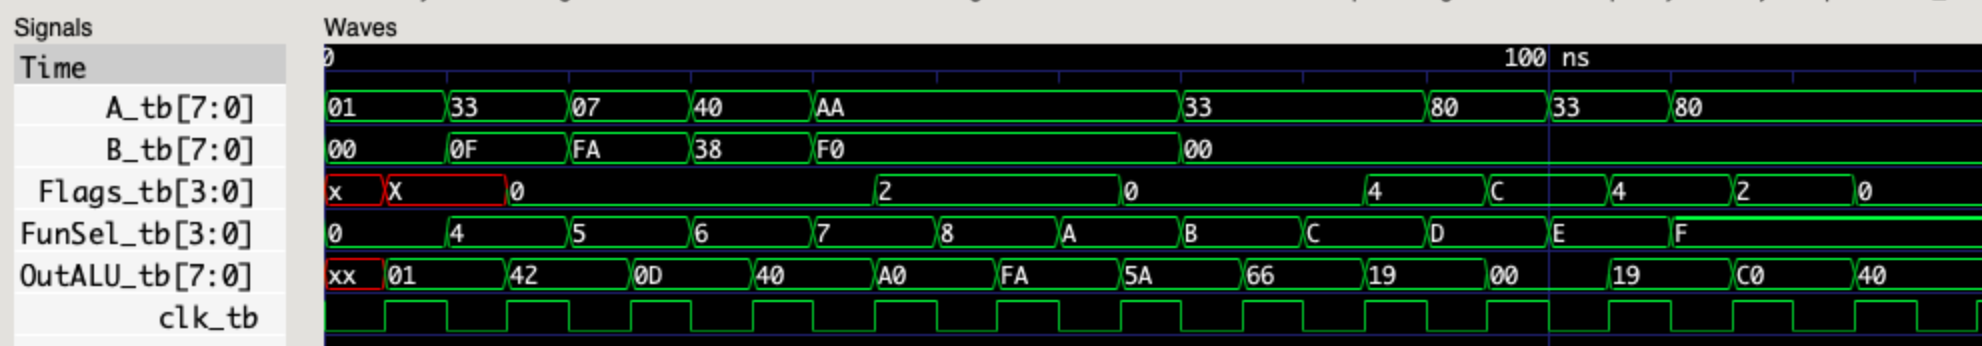
\includegraphics[width=1\textwidth]{part3_sim.png}
\caption{Simulation of Part 3, ALU Module.}
\label{fig:part3_sim}
\end{figure}
\pagebreak
\section{Part 4}
Combining all the module to implement a complete ALU System. \hyperref[fig:part4_diagram]{Figure \ref{fig:part4_diagram}} Shows the diagram of the system implement in this part.

\begin{figure}[H]
\centering
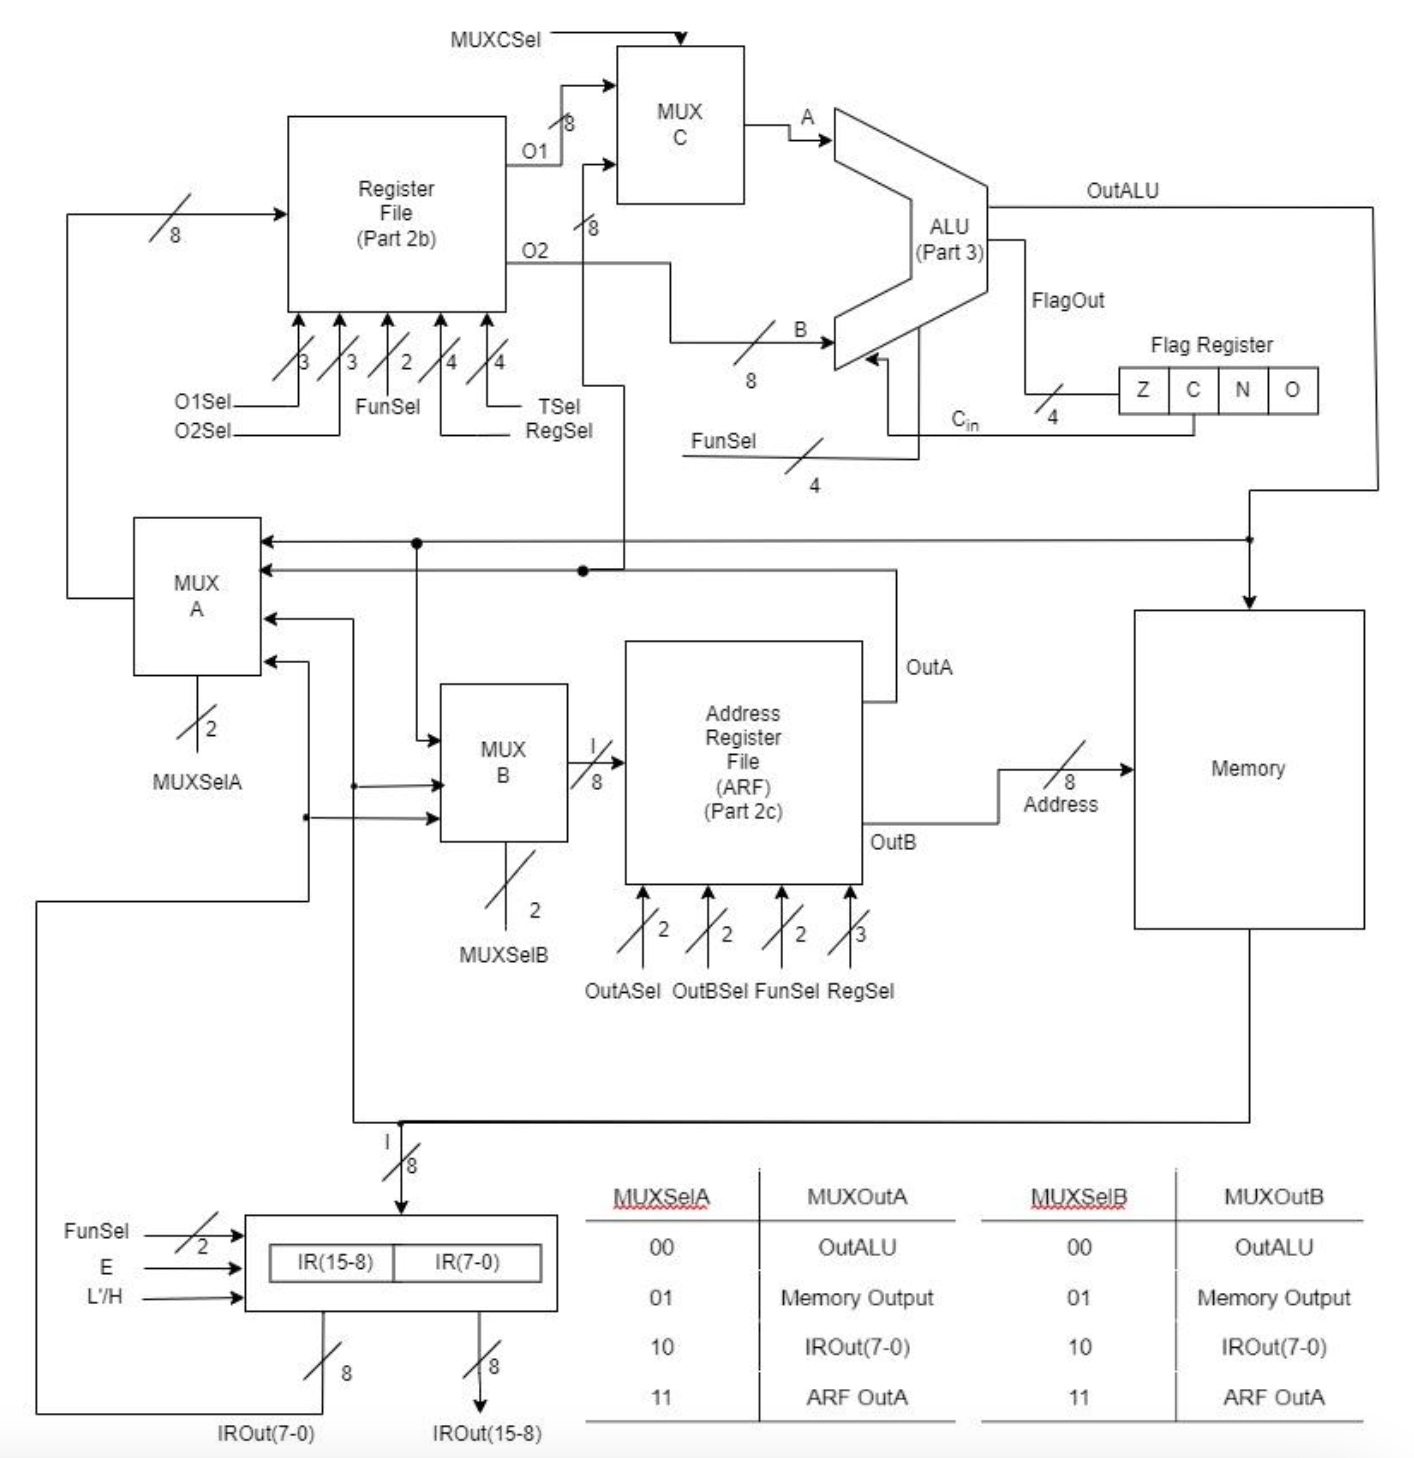
\includegraphics[width=0.8\textwidth]{part4_diagram.png}
\caption{Diagram of the ALU System}
\label{fig:part4_diagram} 
\end{figure}

\subsection{Implementation}
We can implement the system by combining all the module implement by implementing all the previous module in the module as shown:

\begin{lstlisting}
module ALUSystem( input[2:0] RF_O1Sel, input[2:0] RF_O2Sel, input[1:0] RF_FunSel, input[3:0] RF_RSel, input[3:0] RF_TSel, input[3:0] ALU_FunSel, input[1:0] ARF_OutASel, input[1:0] ARF_OutBSel, input[1:0] ARF_FunSel, input[3:0] ARF_RSel, input IR_LH, input IR_Enable, input[1:0] IR_FunSel, input Mem_WR, input      Mem_CS, input[1:0] MuxASel, input[1:0] MuxBSel, input MuxCSel, input Clock );

    wire [7:0] MemOut;
    wire [7:0] RF_O1,RF_O2;
    wire [7:0] MuxAOut, MuxBOut, MuxCOut;
    wire [3:0] ALU_FlagOut;
    wire [7:0] ALU_Out;
    wire [7:0] ARF_OutA, ARF_OutB;
    wire [15:0] IR_Out;
    
    part2c_ARF ARF(Clock, MuxBOut, ARF_OutASel, ARF_OutBSel, ARF_FunSel, ARF_RSel, ARF_OutA, ARF_OutB);

    mux_4to1 MuxA(Clock, MuxASel, ALU_Out, MemOut, IR_Out[7:0], ARF_OutA, MuxAOut);

    mux_4to1 MuxB(Clock, MuxBSel, ALU_Out, MemOut, IR_Out[7:0], ARF_OutA, MuxBOut);

    part2b_RF RF(Clock, MuxAOut, RF_O1Sel, RF_O2Sel, RF_FunSel, RF_RSel, RF_TSel, RF_O1, RF_O2);

    mux_2to1 MuxC(Clock, MuxCSel, RF_O1, ARF_OutA, MuxCOut);

    part3_ALU ALU(Clock, MuxCOut, RF_O2, ALU_FunSel, ALU_Out, ALU_FlagOut);

    Memory Mem(Clock, ARF_OutB, ALU_Out, Mem_WR, Mem_CS, MemOut);

    part2a_IRreg IR(Clock, MemOut, IR_FunSel, IR_LH, IR_Enable, IR_Out);

endmodule
\end{lstlisting}

\subsection{Simulation}
By using the TestBench supplied with the Project, we get the following results shown in \hyperref[fig:part4_sim]{Figure \ref{fig:part4_sim}} when entering the following inputs:
\pagebreak
\begin{lstlisting}
inputs:
1_111_111_11_1111_1111_1111_11_11_11_1111_1_1_10_1_1_11_11_1
1_101_111_11_1111_1111_1111_11_11_11_1111_1_1_11_1_1_11_11_1
0_000_000_00_1111_1111_0000_00_00_00_1111_1_1_00_0_1_11_11_1
1_100_101_01_1100_0000_0011_11_11_11_1111_0_0_00_0_1_11_01_1
1_100_110_01_1010_0000_1100_11_11_11_1101_0_0_00_0_1_11_11_1
1_111_111_11_1111_1101_1111_11_11_11_1111_1_1_01_1_1_11_11_1
1_111_111_11_1111_1111_1111_11_11_11_1011_1_1_11_1_1_11_11_1
\end{lstlisting}

\begin{figure}[H]
\centering
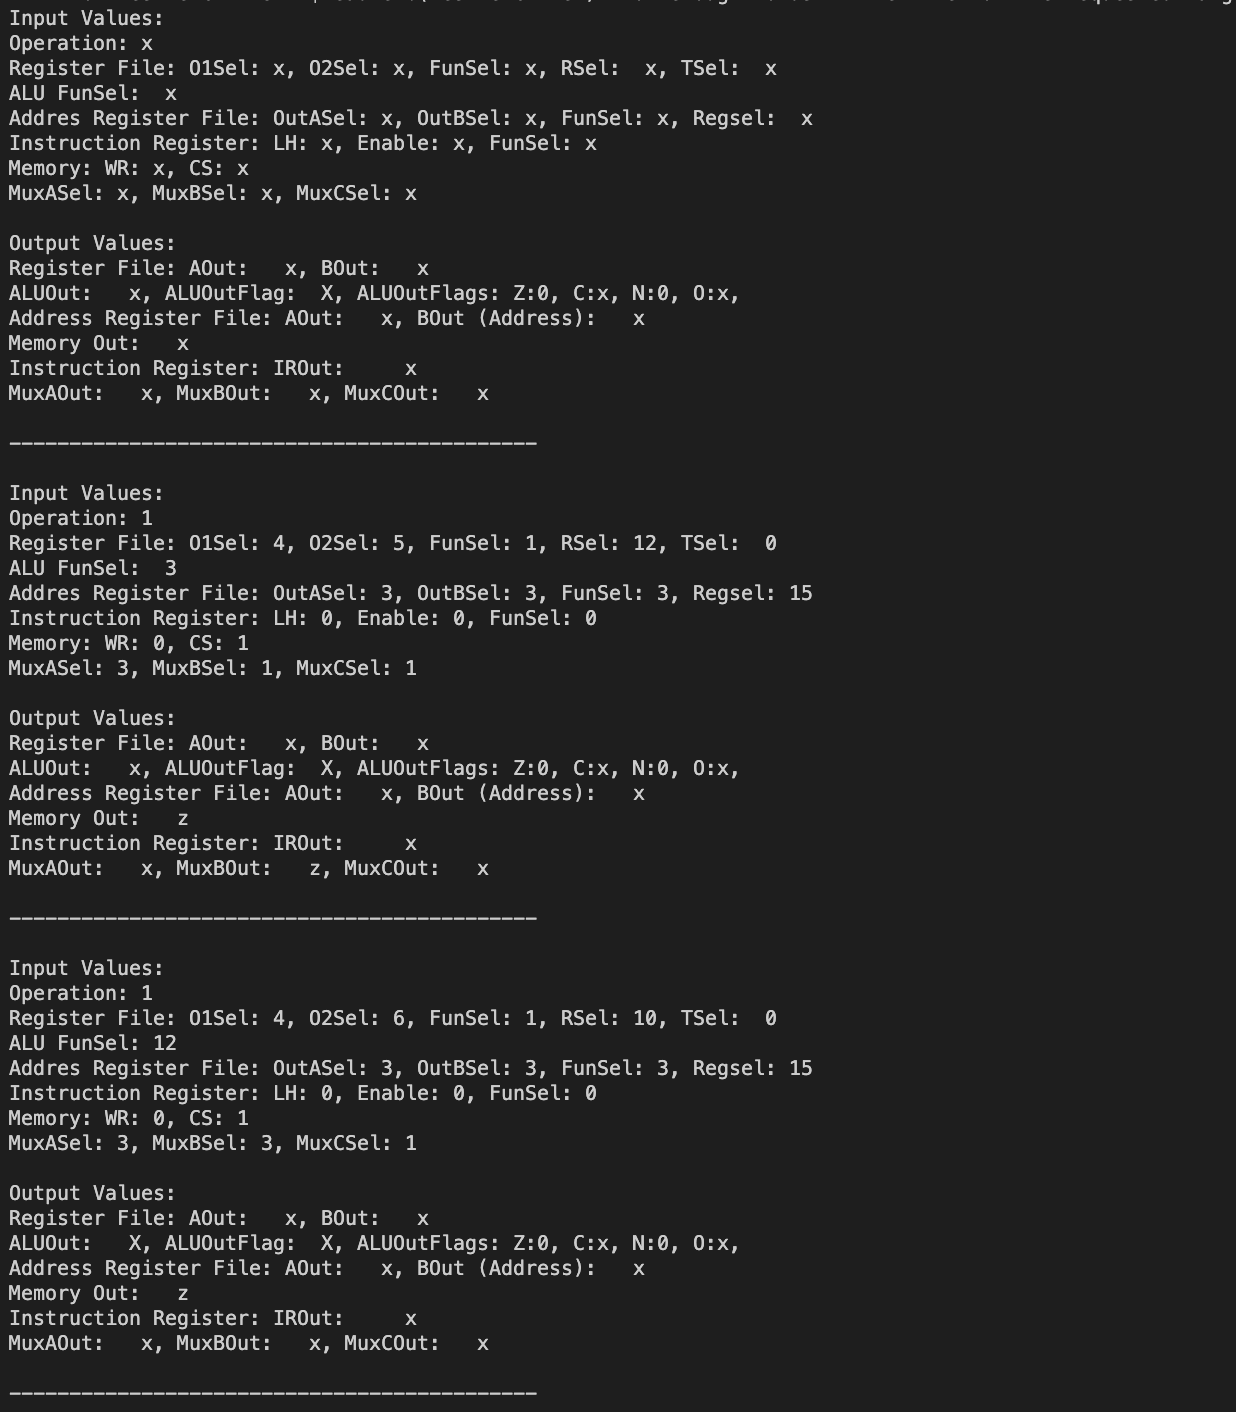
\includegraphics[width=1\textwidth]{part4_sim.png}
\caption{Last 3 results of the simulation of Part 4}
\label{fig:part4_sim}
\end{figure}

\end{document}